
\pagebreak	
\section{Le planning}
\label{bkm:Ref445400921}
Dans la version actuelle de CUBE PA vous pouvez télécharger des plannings (par exemple en tant que fichiers PDF) et les rendre accessibles pour les collaborateurs du projet qui utilisent CUBE PA.
Comme deuxième fonctionnalité du planning, vous pouvez importer des plannings complexes produits avec Microsoft Project en tant que fichiers .xml et puis les filtrer dans CUBE PA et générer des vues spécifiques aux utilisateurs.

%Die Terminplanung beschränkt sich in dern aktuellen CUBE PA Version auf das Herunterladen des Gesamtterminprogramms und das Studienauftragsverfahren Bhf WB, sowie die Filterung und entsprechenden Anzeige des Detailterminprogramms.

\subsection{La visualisation du planning}

\begin{wrapfigure}[8]{l}{6.5cm}   % [x] Wie manche Zeile soll sich um die Grafik "brechen"
  \vspace{-35pt}      % Grundwert war 20; mit 30 schön oben beim Text ausgerichtet
  \begin{center}
    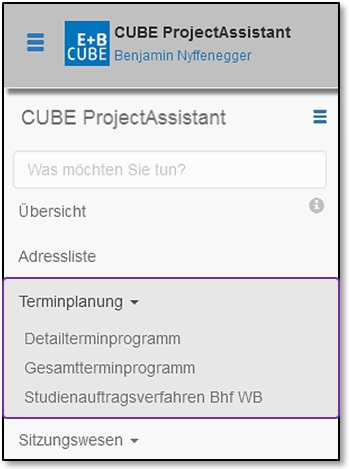
\includegraphics[width=1\linewidth]{../chapters/04_Terminplanung/pictures/4-1_Menu_Terminplanung.jpg}
  \end{center}
  \vspace{-20pt}
  \caption{Utilisation du planning}
  \vspace{-10pt}
\end{wrapfigure}

Dans le menu principal à gauche, choisissez l'élément de menu 'Planning' et ensuite le sous-élément désiré (en cliquant sur 'Planning', les sous-éléments sont affichés ou masqués). La fonction de planning permet d'ajouter des plannings spécifiques au client. Pour cette raison, il est possible que le menu vous paraisse différent par rapport à ce qui présenté dans ce manuel.

\vspace{5cm} 

%\subsection{Das Gesamtterminprogramm und das Studienauftragsverfahren Bhf WB}

%Wenn Sie im Menü unter Terminplan den Unterpunkt 'Gesamtterminprogramm' auswählen, erscheint folgende Ansicht (Diese Ansicht ist abhängig von der CUBE PA-Konfiguration):
% kundenspezifisch
%\begin{figure}[H]
%\center{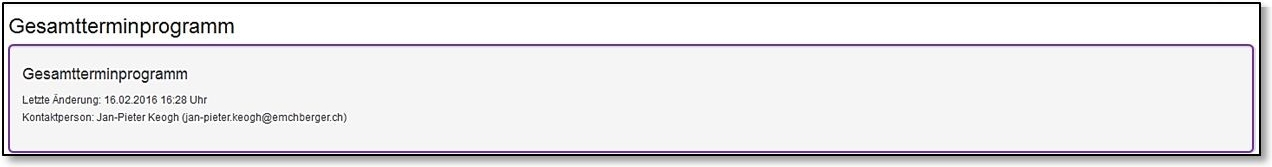
\includegraphics[width=1\linewidth]{../chapters/04_Terminplanung/pictures/4-2_Gesamtterminprogramm.jpg}}
%\caption{Gesamtterminprogramm}
% \label{fig:speciation}
%\end{figure}

%Klicken Sie in den violett umrahmten Bereich, um das Gesamtterminprogramm herunterzuladen. Im nächsten Fenster können Sie wählen, ob das Dokument geöffnet werden soll oder ob Sie es an einem beliebigen Ort abspeichern wollen.

%\vspace{\baselineskip}

%Wenn Sie im Menü unter Terminplan den Unterpunkt 'Studienauftragsverfahren Bhf WB' auswählen, erscheint folgende Ansicht:

% kundenspezifisch
%\begin{figure}[H]
%\center{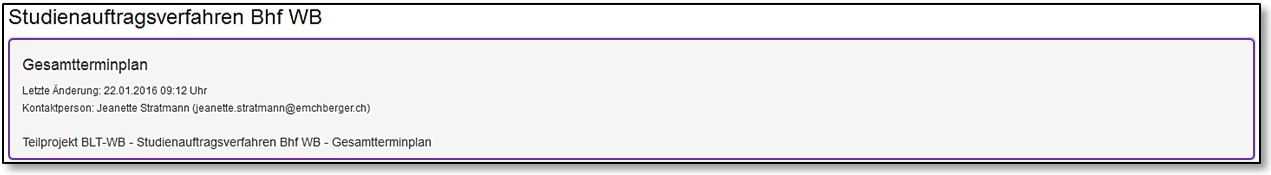
\includegraphics[width=1\linewidth]{42_Studienauftragsv.jpg}}
%\caption{Studienauftragsverfahren Bhf WB}
% \label{fig:speciation}
%\end{figure}

%Klicken Sie in den violett umrahmten Bereich, um das Studienauftragsverfahren Bhf WB herunterzuladen. Im nächsten Fenster können Sie wählen, ob das Dokument geöffnet werden soll oder ob Sie es an einem beliebigen Ort abspeichern wollen.

\subsection{Planning détaillé}

Sélectionnez le sous-élément 'Planning détaillé'. La fenêtre suivante s'affiche, dans laquelle vous pouvez saisir les critères de filtre désirés :

\begin{figure}[H]
\center{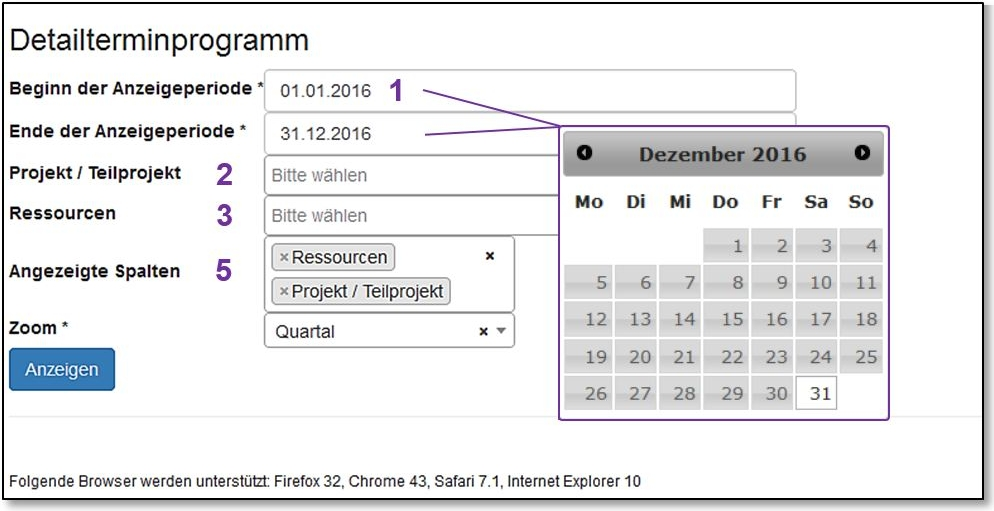
\includegraphics[width=.75\linewidth]{../chapters/04_Terminplanung/pictures/4-3_Detailterminprogramm.jpg}}
\caption{Planning détaillé}
% \label{fig:speciation}
\end{figure}

Les champs marqués par un * sont des champs obligatoires et doivent être remplis. Choisissez le début et la fin de la période pour laquelle vous voulez visualiser le planning \col{(1)}. Un calendrier s'affiche, dans lequel vous pouvez sélectionner la date désirée. Comme option, vous pouvez choisir une projet / sous-projet \col{(2)} et aussi des ressources \col{(3)}.

\begin{figure}[H]
\center{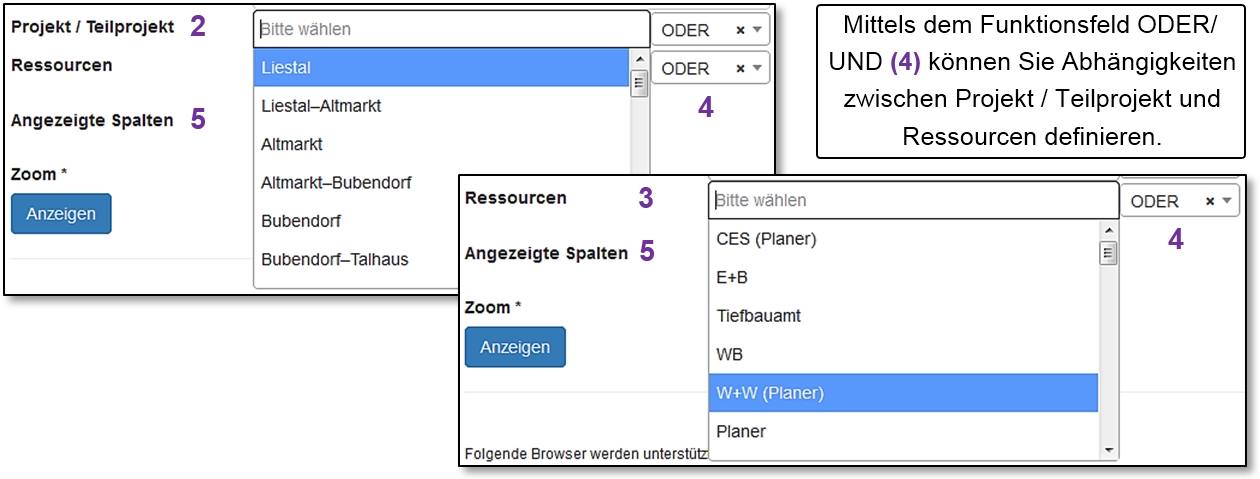
\includegraphics[width=1\linewidth]{../chapters/04_Terminplanung/pictures/4-3_Termine_Abhaengigkeiten.jpg}}
\caption{Définition des dépendances}
% \label{fig:speciation}
\end{figure}

% Text als Grafik implementiert
% Mittels dem Funktionsfeld ODER/UND \textbf{\textcolor[rgb]{0.4392157,0.1882353,0.627451}{(4)}} können Sie Abhängigkeiten zwischen Projekt / Teilprojekt und Ressourcen definieren.

Sélectionnez les colonnes (projet, sous-projet, ressources) à afficher dans les résultats filtrés \col{(5)}. Vous pouvez aussi choisir une deuxième colonne en cliquant à nouveau dans le champ 'Colonnes affichées'. Pour filtrer par projet / sous-projet ou ressource et pour afficher les colonnes dans le plannings, les informations correspondantes doivent être disponibles dans le fichier MS Project (voir chapitre \ref{bkm:Ref445411998}).

% Ref einfügen nach 12.1

\vspace{\baselineskip}

\begin{wrapfigure}[4]{r}{6cm}
  \vspace{-30pt}
  \begin{center}
    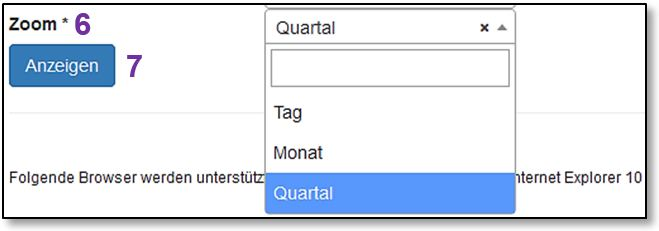
\includegraphics[height=25mm]{43_Zoom-Ansicht.jpg}
  \end{center}
  \vspace{-20pt}
  \caption{Vue agrandie}
  \vspace{-10pt}
\end{wrapfigure}
Sous 'zoom' \col{(6)} vous pouvez choisir si vous voulez une vue de la journée, du mois, ou du trimestre. Une fois les critères de filtrage désirés sont choisis, cliquez 'Afficher' \col{(7)}.

\vspace{\baselineskip}
\vspace{\baselineskip}

Après avoir cliqué sur 'Afficher', le résultat filtré du calendrier est affiché :

\begin{figure}[H]
\center{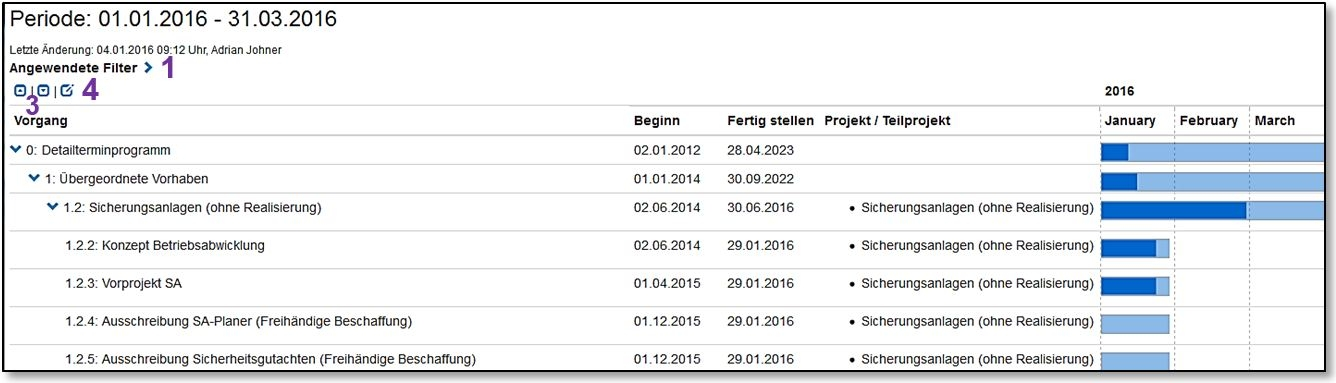
\includegraphics[width=1\linewidth]{43_Termin_Ergebnis.jpg}}
\caption{Résultats du planning}
% \label{fig:speciation}
\end{figure}

Cliquez sur la flèche 
\includegraphics[height=12pt]{/Icons/Pfeil_rechts.jpg} \col{(1)} pour afficher le filtre utilisé. Cliquez à nouveau sur la flèche 
\includegraphics[height=12pt]{/Icons/Pfeil_unten.jpg} \col{(2)} pour masquer le filtre.

\begin{figure}[H]
\center{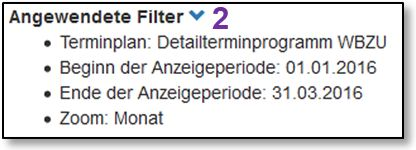
\includegraphics[width=.4\linewidth]{43_Termin_Filter.jpg}}
\caption{Filtre utilisé}
% \label{fig:speciation}
\end{figure}

Avec les deux flèches 
\includegraphics[height=12pt]{/Icons/Pfeil_auf-ab.jpg} \col{(3)} vous pouvez afficher et masquer tous les détails. Pour ajuster les critères de filtrage, cliquez sur le symbole de modification 
\includegraphics[height=12pt]{/Icons/Bearbeiten.jpg} \col{(4)}.
